\documentclass[journal]{vgtc}                     % final (journal style)
%\documentclass[journal,hideappendix]{vgtc}        % final (journal style) without appendices
%\documentclass[review,journal]{vgtc}              % review (journal style)
%\documentclass[review,journal,hideappendix]{vgtc} % review (journal style)
%\documentclass[widereview]{vgtc}                  % wide-spaced review
%\documentclass[preprint,journal]{vgtc}            % preprint (journal style)


%% Uncomment one of the lines above depending on where your paper is
%% in the conference process. ``review'' and ``widereview'' are for review
%% submission, ``preprint'' is for pre-publication in an open access repository,
%% and the final version doesn't use a specific qualifier.

%% If you are submitting a paper to a conference for review with a double
%% blind reviewing process, please use one of the ``review'' options and replace the value ``0'' below with your
%% OnlineID. Otherwise, you may safely leave it at ``0''.
\onlineid{0}

%% In preprint mode you may define your own headline. If not, the default IEEE copyright message will appear in preprint mode.
%\preprinttext{To appear in IEEE Transactions on Visualization and Computer Graphics.}

%% In preprint mode, this adds a link to the version of the paper on IEEEXplore
%% Uncomment this line when you produce a preprint version of the article 
%% after the article receives a DOI for the paper from IEEE
%\ieeedoi{xx.xxxx/TVCG.201x.xxxxxxx}

%% declare the category of your paper, only shown in review mode
\vgtccategory{Research}

%% please declare the paper type of your paper to help reviewers, only shown in review mode
%% choices:
%% * algorithm/technique
%% * application/design study
%% * evaluation
%% * system
%% * theory/model
\vgtcpapertype{please specify}

%% Paper title.
\title{ggdist: Visualizations of Distributions and\\Uncertainty in the Grammar of Graphics}

%% Author ORCID IDs should be specified using \authororcid like below inside
%% of the \author command. ORCID IDs can be registered at https://orcid.org/.
%% Include only the 16-digit dashed ID.
\author{%
  \authororcid{Matthew Kay}{0000-0001-9446-0419}
}

\authorfooter{
  %% insert punctuation at end of each item
  \item
  	Matthew Kay is with Northwestern University.
  	E-mail: mjskay@northwestern.edu
}

%% Abstract section.
\abstract{%
  \lipsum[1] % filler text. Replace with your abstract.
  %
  %% We recommend that you link to your supplemental material here in the abstract, as well
  %% as in the Supplemental Materials section at the end.
  A free copy of this paper and all supplemental materials are available at \url{https://OSF.IO/2NBSG}.
}

%% Keywords that describe your work. Will show as 'Index Terms' in journal
%% please capitalize first letter and insert punctuation after last keyword
\keywords{Uncertainty visualization, distributions, grammar of graphics}

%% A teaser figure can be included as follows
\teaser{
  \centering
  \includegraphics[width=\linewidth]{CypressView}
  \caption{%
  	In the Clouds: Vancouver from Cypress Mountain.
  	Note that the teaser may not be wider than the abstract block.%
  }
  \label{fig:teaser}
}

%% Uncomment below to disable the manuscript note
%\renewcommand{\manuscriptnotetxt}{}

%% Copyright space is enabled by default as required by guidelines.
%% It is disabled by the 'review' option or via the following command:
%\nocopyrightspace


%%%%%%%%%%%%%%%%%%%%%%%%%%%%%%%%%%%%%%%%%%%%%%%%%%%%%%%%%%%%%%%%
%%%%%%%%%%%%%%%%%%%%%% LOAD PACKAGES %%%%%%%%%%%%%%%%%%%%%%%%%%%
%%%%%%%%%%%%%%%%%%%%%%%%%%%%%%%%%%%%%%%%%%%%%%%%%%%%%%%%%%%%%%%%

%% Tell graphicx where to find files for figures when calling \includegraphics.
%% Note that due to the \DeclareGraphicsExtensions{} call it is no longer necessary
%% to provide the the path and extension of a graphics file:
%% \includegraphics{diamondrule} is completely sufficient.
\graphicspath{{figs/}{figures/}{pictures/}{images/}{./}} % where to search for the images

%% Only used in the template examples. You can remove these lines.
\usepackage{tabu}                      % only used for the table example
\usepackage{booktabs}                  % only used for the table example
\usepackage{lipsum}                    % used to generate placeholder text
\usepackage{mwe}         % used to generate placeholder figures
\usepackage{amsmath}
\usepackage{verbatim}
\usepackage{varwidth}

%% We encourage the use of mathptmx for consistent usage of times font
%% throughout the proceedings. However, if you encounter conflicts
%% with other math-related packages, you may want to disable it.
\usepackage{mathptmx}                  % use matching math font

\newenvironment{centerverbatim}{%
  \hfill\break
  \small
  \centering
  \varwidth{\linewidth}%
  \verbatim
}{%
  \endverbatim
  \endvarwidth
  \par
  \hfill\break
}
\newcommand{\dollar}{\$}

\begin{document}

%%%%%%%%%%%%%%%%%%%%%%%%%%%%%%%%%%%%%%%%%%%%%%%%%%%%%%%%%%%%%%%%
%%%%%%%%%%%%%%%%%%%%%% START OF THE PAPER %%%%%%%%%%%%%%%%%%%%%%
%%%%%%%%%%%%%%%%%%%%%%%%%%%%%%%%%%%%%%%%%%%%%%%%%%%%%%%%%%%%%%%%

%% The ``\maketitle'' command must be the first command after the
%% ``\begin{document}'' command. It prepares and prints the title block.
%% the only exception to this rule is the \firstsection command
\firstsection{Introduction}

\maketitle


%% \section{Introduction} %for journal use above \firstsection{..} instead

Uncertainty visualization, generally speaking, has only basic support in existing implementations of the grammar of graphics. Popular implementations like \textit{ggplot2}, \textit{Vega-lite}, and \textit{Observable Plot} typically provide versions of error bars (for points), uncertainty bands (for lines), boxplots, and density plots. Research in uncertainty visualization has long revealed problems with all of these representations and proposed a variety of alternative uncertainty representations to replace them. Examples include quantile dotplots, gradient error bars, gradient plots, gradient bands, and eye plots. Yet, most of these alternative representations are---simply put---painful to convince existing grammar of graphics implementations to produce.

\textit{ggdist} is an attempt to rectify this situation. It started under the guise of \textit{tidybayes}---an R package I wrote for post-processing Bayesian models for use with \textit{ggplot2}---in about 2016. I published \textit{tidybayes} to CRAN (the Comprehensive R Archive Network) in 2018, and it slowly gained some use in the Bayesian statistics community. However, the package had two complementary, but not always perfectly aligned, use cases: post-processing Bayesian model output for visualization, and uncertainty visualization in the grammar of graphics. The latter is bigger than \textit{just} Bayesian statistics: everyone needs to visualize uncertainty! And, contrary to popular opinion---as I'll demonstrate later---Bayesian and frequentist uncertainty visualization can in fact be done within the same framework. Recognizing this broader need, in 2020 I spun off the uncertainty visualization components of \textit{tidybayes} into a new package, \textit{ggdist}, and published it to CRAN. Since then it has steadily grown in use inside and outside the Bayesian statistics community in R, and now averages about 14,000 downloads per month (best described as ``modest'' for an R package).

Over the course of its continuing development, I have learned a lot about how to integrate uncertainty visualization into the grammar of graphics, and developed a formal way of describing that integration (more on that later). In the spirit of recent retrospectives on visualization system design~\textbf{CITE}, I'd like to distill down some of what I've learned here.\footnote{And in the spirit of this being a retrospective, I'm keeping the tone informal. I think that's more honest; and besides, after two years of a pandemic, I at least need a break from stilted academic writing. I hope you do too! If not, whatever.} Ultimately, what would be nice to have---and what I hope to demonstrate \textit{ggdist} to be---is a coherent extension to the grammar of graphics that makes it easy to create the various proposed alternative uncertainty visualizations from the literature, \textit{and more}. By  ``and more'' I mean: not only should we be able to express a variety of uncertainty visualizations through a single coherent framework, but that framework should be complete enough that someone else can wander along and express new uncertainty visualization types I've never thought of before (emphasis on \textit{I}---I think a formalism and its corresponding \textsc{api} truly shows its power when people make things with it that its creator has never thought of before). I'll do this by grounding the design of \textit{ggdist} in a formal representation of uncertainty through mappings of functions of distributions onto visual channels or \textit{aesthetics}. As time is a straight arrow, I can't provide direct evidence that there are visualization types I've never seen before that can be created with \textit{ggdist}, but I will describe instances in which I have encountered uncertainty visualizations in the literature and subsequently realized they were straightforward to express in \textit{ggdist}.

Ultimately, given the huge expressive power of the grammar of graphics and the popularity of tools built on it, I hope a catalog of my experiences here might provide a catalyst for improved implementations of uncertainty visualization to flourish in existing grammar of graphics ecosystems. Let's give it a try.

\section{Setting the stage}

\subsection{A simplified notation for the grammar of graphics}

To be able to talk more generally than a specific grammar of graphics implementation, we'll at least need a formal way of writing down visualization specifications separated from a particular implementation. I'll adopt here a notation that I've found works pretty well when I teach the grammar of graphics to undergraduates. I've used a variation on this notation when teaching \textit{ggplot2}, \textit{Vega-lite}, \textit{Altair}, and \textit{Tableau} and found students pick it up easily, which is at least some evidence it might be easy for folks to understand. The core notation describes a visualization in terms of its \textit{data variables}, \textit{aesthetic mappings}, and \textit{geometries}. We create a scatterplot, for example, by mapping one variable onto the \textit{x} aesthetic and another onto the \textit{y} aesthetic:

\hfill\break
  \begin{minipage}{.5\columnwidth}
    \begin{align*}
\mathit{weight} &\rightarrow x\\
\mathit{mpg} &\rightarrow y\\
\textsc{geom} &= \mathit{point}
\end{align*}
  \end{minipage}%
  \begin{minipage}{.4\columnwidth}
    \centering
    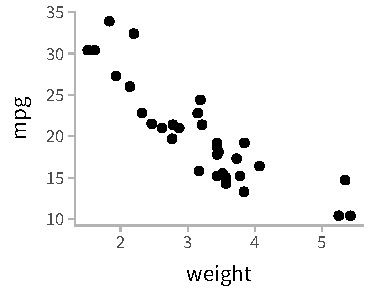
\includegraphics[width=1.2\columnwidth]{figs/2-mpg_v_weight.pdf}
  \end{minipage}


This notation sets up two \textit{aesthetic mappings}:\footnote{Or in \textit{Vega-lite} parlance, \textit{encodings}} a mapping from the \textit{weight} data variable onto the \textit{x} aesthetic, and a mapping from the \textit{mpg} data variable onto the \textit{y} aesthetic. It then employs a \textit{point} geometry\footnote{\textit{Vega-lite}-ese: mark} for display. I like this notation because it emphasizes that we are creating \textit{functions} from data space to aesthetic (display) space; in grammar of graphics parlance these are \textit{scale} functions which can themselves be specified (e.g., to set up log scales, to pick how colors are assigned to data values, etc). Other notations obscure this key insight into the structure of the grammar of graphics by, e.g., placing the aesthetic first and ``assigning'' data variables to it, which gives an incorrect intuition in my view. In fact, let's see that now: here is a translation of the above into \textit{ggplot2} code, assuming \texttt{cars} is a data frame with \texttt{weight} and \texttt{mpg} columns:

\begin{centerverbatim}
ggplot(cars) +
  aes(
    x = weight,
    y = mpg
  ) +
  geom_point()
\end{centerverbatim}

Or in \textit{Vega-lite}:\footnote{I use the Vega-lite \textsc{api} instead of its \textsc{json} form, as \textsc{json} is a horrifying mess of visual noise, and no sane human should want to read or write it. The Vega-lite \textsc{api} is a notable improvement, though without R's facility for capturing and re-writing abstract syntax trees, it can't quite reach the succinctness of \textit{ggplot2}---though this is a fundamental limitation of trying to write domain-specific languages in JavaScript, and no fault of the \textit{Vega-lite} authors, who have done an excellent job with the language they've been given.}

\begin{centerverbatim}
vl.data("path/to/cars.json")
  .encode(
    vl.x().fieldQ("weight"),
    vl.y().fieldQ("mpg")
  )
  .markPoint()
\end{centerverbatim}

This shows the close correspondence between the abstract notation above and the particulars of code in actual grammar of graphics implementations. Throughout the rest of this paper, I'll stick to the abstract notation and corresponding \textit{ggplot2} + \textit{ggdist} code for the particulars.

\subsection{Uncertainty visualization in the grammar of graphics, as she is spoke}

Speaking of existing implementations of the grammar of graphics, how do they implement uncertainty visualization? Rudimentarily, I would argue.

One natural approach to uncertainty visualization is to assume a Gaussian approximation: to represent all estimates and their uncertainty as a mean and standard deviation. This makes the specification problem easy: instead of mapping a single value onto the \textit{x} aesthetic, say, we map a point estimate onto \textit{x} and provide an aesthetic for its standard deviation; call it $x_\textsc{sd}$. Say we had estimated a variable $a$ and had quantified its standard error (i.e. the standard deviation of its sampling distribution) as $\sigma_a$, we might plot a point with an error bar using a \textit{pointinterval} geometry as follows, yielding a 95\% interval calculated from a Normal distribution with mean $a$ and standard deviation $\sigma_a$:

\hfill\break
  \begin{minipage}{.5\columnwidth}
\begin{align*}
a &\rightarrow x\\
\sigma_a &\rightarrow x_\textsc{sd}\\
\textsc{geom} &= \mathit{pointinterval}
\end{align*}
  \end{minipage}%
  \begin{minipage}{.4\columnwidth}
    \centering
    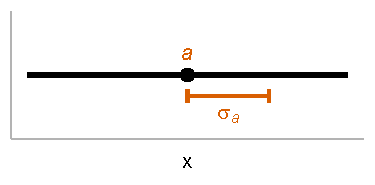
\includegraphics[width=1.2\columnwidth]{figs/2-mean_sd_interval.pdf}
  \end{minipage}

This is one approach taken by \textit{Vega-lite}: it provides an \texttt{errorbar}\footnote{\texttt{errorbar} is, in my view, a misnomer, as is \texttt{xError}: fundamentally, the mark calculates a Gaussian interval, which might be for a distribution being used to represent error in an estimate, but might not. \textit{Error} is not the generic notion at play; a standard deviation is; and the generic mark is an interval, not an error bar.} mark (analogous to \textit{pointinterval}) and an \texttt{xError}  channel (analogous to $x_\textsc{sd}$). I'll refer to this notation as the $\{x, x_\textsc{sd}\}$ approach.

The problem, fundamentally, is that not all uncertainty is well-represented by a Gaussian distribution. Consider uncertainty in a proportion (bounded at 0 and 1, thus as estimates approach the boundary the interval becomes asymmetric---yet Gaussian intervals must be symmetric) or uncertainty in a variance parameter (bounded below at 0). Or, consider the ubiquitous Student-\textit{t} confidence interval: as the degrees of freedom go to $\infty$, a Student-\textit{t} distribution is well approximated by the Normal, but with low degrees of freedom (incidentally common in small-\textit{n} studies---like at \textsc{vis}), the tails of the distribution become fatter, and the Normal distribution is a poor approximation. Thus, a more general approach is needed.

The obvious alternative, at least for interval representations, is to simply specify the endpoints of the intervals; e.g. for a 95\% Gaussian interval:

  \begin{minipage}{.5\columnwidth}
\begin{align*}
a &\rightarrow x\\
a - 1.96 \cdot \sigma_a &\rightarrow x_\textsc{min}\\
a + 1.96 \cdot \sigma_a &\rightarrow x_\textsc{max}\\
\textsc{geom} &= \mathit{pointinterval}
\end{align*}
  \end{minipage}%
  \begin{minipage}{.4\columnwidth}
    \centering
    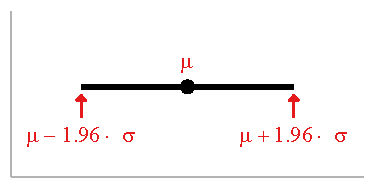
\includegraphics[width=1.2\columnwidth]{figs/2-xmin_xmax_interval.pdf}
  \end{minipage}
\hfill\break

Here, the magic values $-1.96$ and $+1.96$ are the $(1-95\%/2) = 2.5\%$th and $(1+95\%/2) = 97.5\%$th quantiles of the standard Normal distribution, thus yielding a $97.5\% - 2.5\% = 95\%$ interval. This is generic in the sense that any interval can be represented, but unsatisfying in the sense that we seem to have lost some level of abstraction that was present when we were just thinking in terms of estimates and their variances. These also require that the user knows how to make these calculations. Both \textit{ggplot2} (with \texttt{geom\_pointrange}) and \textit{Vega-lite} (with the \texttt{x} and \texttt{x2} channels supplied to \texttt{errorbar}) offer a variant of this solution for pre-calculated intervals. 

I will offer a different solution: to instead represent intervals as properties of a distribution, allowing us to neatly handle both the simple case of Gaussian error and more complex cases. Centering distributions---not standard deviations or intervals---in the specification of uncertainty will also allow us to build a richer set of uncertainty representations.

\section{Uncertainty visualization as distributional visualization}

\subsection{Intervals}

Imagine we represent an uncertain value generically as a distribution, or a random variable, $A$. Importantly, I do not consider this a \textit{probability} distribution necessarily: it could be a probability distribution, but it could also be a \textit{confidence} distribution, which is a frequentist generalization of sampling distributions and bootstrap distributions~\textbf{CITE}. Its defining characteristic will be that it has a cumulative distribution function (\textsc{cdf}), $F_A(x)$, which is:
\begin{itemize}
    \item For a probability distribution, $F_A(x) = \Pr(A \le x)$, the probability that $A$ is less than or equal to $x$.
    \item   For a confidence distribution, $F_A(x) = \gamma$  is the confidence $\gamma$ at which $x$ would be the upper limit of a one-sided $\gamma\%$ confidence interval, $[-\infty, x]$, for $A$. That sentence is pretty typical of convoluted frequentist definitions, so it might be easier to think in terms of the inverse: $F_A^{-1}(\gamma)$ yields the value $x$, which is the upper limit of a one-sided $\gamma\%$ confidence interval on $A$: $[-\infty,x]$. So $[-\infty, F_A^{-1}(0.95)]$ is a one-sided 95\% confidence interval on $A$.
\end{itemize}

For either representation, we may also be interested in other functions of the distribution. These include the derivative of the cumulative distribution function, i.e. the density function (or the mass function, if the distribution is discrete), $f_A(x)$, as well as the inverse of the \textsc{cdf} (also known as the quantile function), $F_A^{-1}(x)$. Given these functions, we can generate a variety of uncertainty representations, including but not limited to density plots and intervals.

For example, a median and $\gamma\%$ quantile interval could be defined generically on any distribution $A$ as follows:

\begin{minipage}{.5\columnwidth}
\begin{align*}
\operatorname{median}(A) &\rightarrow x\\
F_A^{-1}\left(\frac{1 - \gamma}{2}\right) &\rightarrow x_\textsc{min}\\
F_A^{-1}\left(\frac{1 + \gamma}{2}\right) &\rightarrow x_\textsc{max}\\
\textsc{geom} &= \mathit{pointinterval}
\end{align*}
\end{minipage}%
  \begin{minipage}{.4\columnwidth}
    \centering
    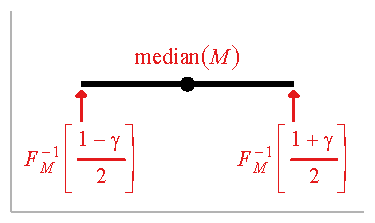
\includegraphics[width=1.2\columnwidth]{figs/3-geom_pointinterval_quantiles.pdf}
  \end{minipage}
\hfill\break

If $A$ is a probability distribution, this is a Bayesian \textit{credible }interval, and if $A$ is a confidence distribution, this is a frequentist \textit{confidence} interval. This lets us abstract over the petty battles between this or that statistical camp and get to the meaningful business of visualizing uncertainty. This also allows us something not present in other attempts so far: to make it easy to specific multiple interval sizes, and to map interval size itself onto an aesthetic. For example, if we\footnote{Yes yes, I am using both ``I'' and ``we'' in this paper. ``I'' is me, and ``we'' is the conspiratorial ``we'': I'd like to hope you'll come with me on the journey of trying to sort out reasonable ways of visualizing uncertainty.} wanted to show two intervals, a 95\% and a 66\%, where the smaller interval is shown as a thicker line, we could write:

\begin{minipage}{.5\columnwidth}

\begin{align*}
\operatorname{median}(A) &\rightarrow x\\
F_A^{-1}\left(\frac{1 - \gamma}{2}\right) &\rightarrow x_\textsc{min}\\
F_A^{-1}\left(\frac{1 + \gamma}{2}\right) &\rightarrow x_\textsc{max}\\
-\gamma &\rightarrow \mathit{linewidth}\\
\textsc{geom} &= \mathit{pointinterval}\\
\gamma &\in \{0.66, 0.95\}
\end{align*}
\end{minipage}%
  \begin{minipage}{.4\columnwidth}
    \centering
    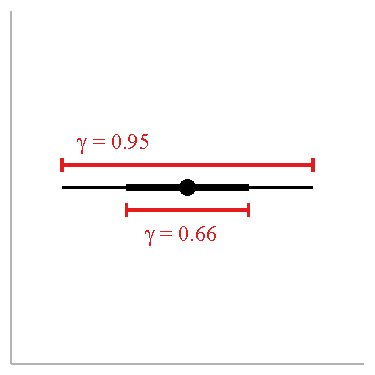
\includegraphics[width=1.2\columnwidth]{figs/3-stat_pointinterval_linewidth.pdf}
  \end{minipage}
\hfill\break

This is a not uncommon approach that tries to avoid dichotomous thinking by showing multiple intervals of different masses. It also has the nice grammar-of-graphics-ish property of mapping the mass ($\gamma$) onto the width of the line, instead of creating two explicit, separate layers, each specifying a different interval---it makes the mass into \textit{data}.\footnote{I learned at least two useful things from a relational databases class in undergrad: (1) it's always better to put data into rows than into column names of tables---an insight that stems from database \textit{normal forms}~\textbf{CITE} (distinctions between which I have long forgotten) or what some statisticians call \textit{tidy data}~\textbf{CITE}; and (2) you are rarely at Google scale, so you're probably better off with a relational database with proper transactions than some dumb old key value store. The latter lesson my grad students refuse to learn until they build a webapp to collect data from 300 participants using some newfangled database they aren't the target users for, and end up with garbage. Kids these days, etc.} This also makes it easy to generalize to other visualizations, e.g. by modifying the previous specification to map mass onto \textit{color} instead of \textit{linewidth}:


\begin{minipage}{.5\columnwidth}

\begin{align*}
-\gamma &\rightarrow \mathit{color}\\
\textsc{geom} &= \mathit{pointinterval}\\
\gamma &\in \{0.50, 0.80, 0.95\}
\end{align*}
\end{minipage}%
  \begin{minipage}{.4\columnwidth}
    \centering
    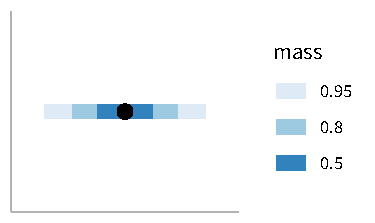
\includegraphics[width=1.2\columnwidth]{figs/3-stat_pointinterval_color.pdf}
  \end{minipage}
\hfill\break


On the other hand, these are still a bit low-level: they require the user to know how to calculate interval endpoints from the quantile function. This also limits us specifically to quantile intervals, when other intervals types, such as highest-density intervals~\textbf{CITE} and shortest intervals~\textbf{CITE}, might be preferable. Thus, \textit{ggdist} also supplies a \textit{stat} version of \textit{pointinterval}, which bundles up some statistical calculations and default aesthetic mappings with the \textit{pointinterval} geometry. All \textit{stat}s in \textit{ggdist} support the $x_\textsc{dist}$ and $y_\textsc{dist}$ aesthetics, onto which objects that represent distributions can be mapped. They also allow the user to specify the type of point and interval used, and generate the corresponding values and mappings for $x$, $x_\textsc{min}$, $x_\textsc{max}$, and \textit{linewidth}. This changes the specification to something like:


\begin{minipage}{.5\columnwidth}

\begin{align*}
A &\rightarrow x_\textsc{dist}\\
\textsc{stat} &= \mathit{pointinterval}\\
\textsc{point} &= \mathit{median}\\
\textsc{interval} &= \textit{quantile interval}\\
\gamma &\in \{0.66, 0.95\}
\end{align*}
\end{minipage}%
  \begin{minipage}{.4\columnwidth}
    \centering
    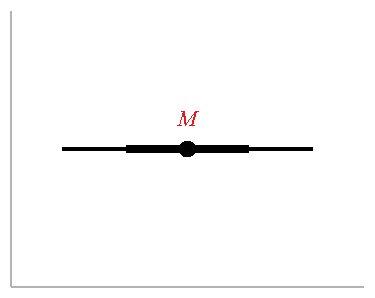
\includegraphics[width=1.2\columnwidth]{figs/3-stat_pointinterval_A.pdf}
  \end{minipage}
\hfill\break

The representation of the distribution $A$ could be a sample-based representation, e.g. a bunch of draws from a Bayesian posterior or from a bootstrap distribution, or it could be an object representing a theoretical distribution in terms of its parameters, such as a Normal distribution with a defined mean and standard deviation. Point estimates and interval types can be defined by arbitrary functions of distributions, and predefined functions for mean, median, and mode, and quantile, highest-density, and shortest intervals are provided. This generalizes the $\{x, x_\textsc{sd}\}$ approach used by \textit{Vega-lite} to any distribution type while abstracting over the specifics of how point estimates and intervals are calculated.

In implementation, \textit{ggdist} allows distributions to be represented by numeric vectors (sample-based representation), objects from the \textit{distributional } R package (which supports theoretical distributions), and \texttt{rvar} objects from the \textit{posterior} R package (a sample-based representation that mimics numeric arrays in R). For example, if we re-create the $\{x, x_\textsc{sd}\}$ representation abstractly thus:

\begin{minipage}{.5\columnwidth}

\begin{align*}
\operatorname{Normal}(a, \sigma_a) &\rightarrow x_\textsc{dist}\\
\textsc{stat} &= \mathit{pointinterval}\\
\textsc{point} &= \mathit{median}\\
\textsc{interval} &= \textit{quantile interval}\\
\gamma &\in \{0.66, 0.95\}
\end{align*}
\end{minipage}%
  \begin{minipage}{.4\columnwidth}
    \centering
    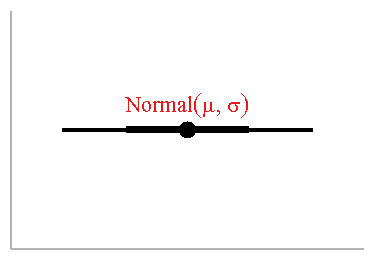
\includegraphics[width=1.2\columnwidth]{figs/3-stat_pointinterval_normal.pdf}
  \end{minipage}
\hfill\break

In \textit{ggdist}, using \texttt{distributional::dist\_normal}, the specification is quite similar:

\begin{centerverbatim}
ggplot(data) +
  aes(xdist = dist_normal(a, sigma_a)) +
  stat_pointinterval(
    point_interval = median_qi, 
    .width = c(.66, .95)
  )
\end{centerverbatim}

These happen to be the default values for \texttt{point\_interval} and \texttt{.width} ($\gamma$),\footnote{For historical reasons that have to do with a combination of a very long discussion with a bunch of people on the Stan forums~\textbf{CITE} and naming conventions in some R \textsc{api}s for fixed arguments to functions with variable argument lists~\textbf{CITE}, $\gamma$ in \textit{ggdist} is spelled \texttt{.width}. Reflecting on my past mistakes, a better name would be  \texttt{mass}.} so just \texttt{stat\_pointinterval()}  also works here. To demonstrate generalizing this approach, consider the very common need of placing uncertainty intervals on the results of a $t$-test, which can be derived from a $t_\nu(\mu, \sigma)$  distribution with $\nu$ degrees of freedom, scale $\mu$ (e.g. an estimated mean), and scale $\sigma$ (e.g. a standard error). Given these three numbers in a data frame, a visualization specification might be:

\begin{minipage}{.5\columnwidth}

\begin{align*}
t_{\nu_a}(a, \sigma_a) &\rightarrow x_\textsc{dist}\\
\textsc{stat} &= \mathit{pointinterval}
\end{align*}
\end{minipage}%
  \begin{minipage}{.4\columnwidth}
    \centering
    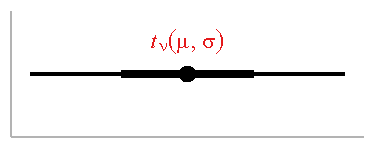
\includegraphics[width=1.2\columnwidth]{figs/3-stat_pointinterval_student_t.pdf}
  \end{minipage}
\hfill\break


Which in \textit{ggdist} is:

\begin{centerverbatim}
ggplot(data) +
  aes(xdist = dist_student_t(nu_a, a, sigma_a)) +
  stat_pointinterval()
\end{centerverbatim}

\subsection{Ribbons}

Once we have \textit{pointinterval} representations, it is straightforward to develop uncertainty band representations by generalizing points to lines and intervals to ribbons---thus, \textit{lineribbon}. Imagine a regression that models car miles per gallon based on weight (the details of the function $g$ are not important):

\[
\log(\mathit{mpg}) \sim \operatorname{Normal}\left(g(\mathit{weight}), \sigma\right)
\]
Such a model could provide a predictive distribution for a car's miles per gallon conditional on its weight: $p(\mathit{mpg} \mid \mathit{weight})$, which we might want to plot alongside the raw data. If a \textit{lineribbon} is a geometry combining a line with an arbitrary number of uncertainty bands around it, abstractly, we want something like this:

\begin{minipage}{.5\columnwidth}

\begin{align*}
\mathit{weight} &\rightarrow x\\
p(\mathit{mpg} \mid \mathit{weight}) &\rightarrow y_\textsc{dist}\\
\gamma &\rightarrow \mathit{fill}\\
\textsc{stat} &= \mathit{lineribbon}\\
\gamma &\in \{0.50, 0.80, 0.95\}
\end{align*}
\end{minipage}%
  \begin{minipage}{.4\columnwidth}
    \centering
    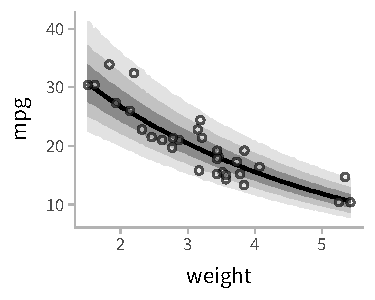
\includegraphics[width=1.2\columnwidth]{figs/3-lineribbon.pdf}
  \end{minipage}
\hfill\break


I include the raw data as a separate \textit{point} geometry layer as well, for comparison. Assuming \texttt{m}  is a Bayesian version of such a model fit using the \textit{brms} modeling package in R, and \texttt{preds} is a data frame of desired \textit{weight} values to predict on, we can add a column to \texttt{preds} that contains a random variable representation of $p(\mathit{mpg} \mid \mathit{weight})$ using \texttt{brms::posterior\_predict}~\textbf{CITE} and the \texttt{posterior::rvar}  data type~\textbf{CITE}. The latter is a data type I created\footnote{This was a slightly insane idea in itself, given the way that base R data types work. As R's classes work based on generic \textit{functions}, rather than classes with a well-defined set of methods, this requires tracking down all the various functions implemented to work with arrays and vectors in the language and providing implementations for them for random variable arrays. Indexing functions especially are annoying, as there are half a dozen different ways to index into R arrays, each with myriad corner cases. Anyway.} specifically to wrap large samples that represent distributions into objects that mimic R vectors and arrays, and which can be added to data frames:

\begin{centerverbatim}
preds = preds |> mutate(
  mpg_given_weight = rvar(posterior_predict(m, preds)
)
\end{centerverbatim}

Given this data frame, we the equivalent of the abstract specification above is:

\begin{centerverbatim}
ggplot(preds) +
  aes(x = weight, ydist = mpg_given_weight) +
  stat_lineribbon()
\end{centerverbatim}

\texttt{stat\_lineribbon} defaults to \texttt{.width = c(.5, .8, .95)} and maps the resulting \texttt{.width} onto the \texttt{fill} aesthetic, so we do not need to specify \texttt{.width} or the \texttt{fill} mapping for this example.

Once we have a multiple-ribbon geometry, it is easy to create other uncertainty visualization types, like gradient fan charts~\textbf{CITE}. For example, we could use a large number of intervals, say $k = 50$ or $100$, and generate $k$  evenly-spaced interval widths between 0 and 1 (not including 0 or 1): $\gamma = \{(1 - 0.5)/k, \dots, (k - 0.5)/k\}$. This is the \texttt{ppoints(k)} function in R, so we can simply write \texttt{stat\_lineribbon(.width = ppoints(100))} to get a gradient fan chart with 100 intervals. This steams directly from my choice to make $\gamma$ into data, and is one example of support for a chart type that was a happy accident of \textit{ggdist}'s design.

 
\section{Hyperlinks and Cross References}

The style uses the \verb|hyperref| package which can typeset clickable hyperlinks using \verb|\href{...}{...}|, hyperlinked URLs using \verb|\url{...}|, and turns references into internal links.

The style also uses \verb|cleveref| to automatically and consistently format cross references.
We recommend that you use the \verb|\cref{label}| and \verb|\Cref{label}| calls instead of \verb|Figure~\ref{label}| or similar.
\verb|\Cref| should be used when starting a sentence to spell out the reference (e.g.\ ``Section'') while \verb|\cref| should be used when referencing within a sentence to abbreviate (e.g.\ ``Sec.'').
Here are examples for use within a sentence: \cref{fig:vis_papers}, \cref{tab:vis_papers}, \cref{sec:supplement_inst,sec:references_inst}, \cref{eq:sum}.
The following sentences all start with a reference, so use \verb|\Cref|.
\Cref{fig:vis_papers} is a \verb|figure| environment.
\Cref{tab:vis_papers} is a \verb|table| environment.
\Cref{sec:supplement_inst,sec:references_inst} are \verb|section| environments.
\Cref{eq:sum} is an \verb|equation| environment.


\section{Figures}

\subsection{Loading figures}

The style automatically looks for image files with the correct extension (eps for regular \LaTeX; pdf, png, and jpg for pdf\LaTeX), in a set of given subfolders defined above using \verb|\graphicspath|: figures/, pictures/, images/.
It is thus sufficient to use \verb|\includegraphics{CypressView}| (instead of \verb|\includegraphics{pictures/CypressView.jpg}|).
Figures should be in CMYK or Grey scale format, otherwise, colour shifting may occur during the printing process.

\subsection{Vector figures}

Vector graphics like svg, eps, pdf are best for charts and other figures with text or lines.
They will look much nicer and crisper and any text in them will be more selectable, searchable, and accessible.

\subsection{Raster figures}

Of the raster graphics formats, screenshots of user interfaces and text, as well as line art, are better shown with png.
jpg is better for photographs.
Make sure all raster graphics are captured in high enough resolution so they look crisp and scale well.

\subsection{Figures on the first page}

The teaser figure should only have the width of the abstract as the template enforces it.
The use of figures other than the optional teaser is not permitted on the first page.
Other figures should begin on the second page.
Papers submitted with figures other than the optional teaser on the first page will be refused.

\subsection{Subfigures}

You can add subfigures using the \texttt{subcaption} package that is automatically loaded.
Inside a \verb|figure| environment, create a \verb|subfigure| environment.
See \cref{fig:ex_subfigs} for an example.
We can reference individual figures, either fully using \verb|\cref| (\cref{fig:ex_subfigs_a,fig:ex_subfigs_b}) or by letter using \verb|\subref|.
E.g., \subref{fig:ex_subfigs_b}, \subref{fig:ex_subfigs_c}.
Note that \verb|\subref| only works for one label at a time.

\begin{figure}[tbp]
  \centering
  \begin{subfigure}[b]{0.45\columnwidth}
  	\centering
  	\includegraphics[width=\textwidth]{example-image-a}
  	\caption{The letter A.}
  	\label{fig:ex_subfigs_a}
  \end{subfigure}%
  \hfill%
  \begin{subfigure}[b]{0.45\columnwidth}
  	\centering
  	\includegraphics[width=\textwidth]{example-image-b}
  	\caption{The letter B.}
  	\label{fig:ex_subfigs_b}
  \end{subfigure}%
  \\%
  \begin{subfigure}[b]{0.45\columnwidth}
  	\centering
  	\includegraphics[width=\textwidth]{example-image-c}
  	\caption{The letter C.}
  	\label{fig:ex_subfigs_c}
  \end{subfigure}%
  \subfigsCaption{Example of adding subfigures with the \texttt{subcaption} package.}
  \label{fig:ex_subfigs}
\end{figure}

\subsection{Figure Credits}
\label{sec:figure_credits_inst}

In the \hyperref[sec:figure_credits]{Figure Credits} section at the end of the paper, authors should credit the original sources of any figures that were reproduced or modified.
Include any license details necessary, as well as links to the original materials whenever possible.
For credits to figures from academic papers, include a citation that is listed in the \textbf{References} section.
An example is provided \hyperref[sec:figure_credits]{below}.

\textbf{For IEEE VIS}, this section may be included in the \textbf{2-page allotment for References, Figure Credits, and Acknowledgments}.



\section{Equations and Tables}

Equations can be added like so:

\begin{equation}
  \label{eq:sum}
  \sum_{j=1}^{z} j = \frac{z(z+1)}{2}
\end{equation}

Tables, such as \cref{tab:vis_papers} can also be included.


\begin{table}[tb]
  \caption{%
  	VIS/VisWeek accepted/presented papers: 1990--2016.%
  }
  \label{tab:vis_papers}
  \scriptsize%
  \centering%
  \begin{tabu}{%
  	  r%
  	  	*{7}{c}%
  	  	*{2}{r}%
  	}
  	\toprule
  	year & \rotatebox{90}{Vis/SciVis} &   \rotatebox{90}{SciVis conf} &   \rotatebox{90}{InfoVis} &   \rotatebox{90}{VAST} &   \rotatebox{90}{VAST conf} &   \rotatebox{90}{TVCG @ VIS} &   \rotatebox{90}{CG\&A @ VIS} &   \rotatebox{90}{VIS/VisWeek} \rotatebox{90}{incl.\ TVCG/CG\&A}   &   \rotatebox{90}{VIS/VisWeek} \rotatebox{90}{w/o TVCG/CG\&A}   \\
  	\midrule
  	2016 & 30 &   & 37 & 33 & 15 & 23 & 10 & 148 & 115 \\
  	2015 & 33 & 9 & 38 & 33 & 14 & 17 & 15 & 159 & 127 \\
  	2014 & 34 &   & 45 & 33 & 21 & 20 &    & 153 & 133 \\
  	2013 & 31 &   & 38 & 32 &    & 20 &    & 121 & 101 \\
  	2012 & 42 &   & 44 & 30 &    & 23 &    & 139 & 116 \\
  	2011 & 49 &   & 44 & 26 &    & 20 &    & 139 & 119 \\
  	2010 & 48 &   & 35 & 26 &    &    &    & 109 & 109 \\
  	2009 & 54 &   & 37 & 26 &    &    &    & 117 & 117 \\
  	2008 & 50 &   & 28 & 21 &    &    &    &  99 &  99 \\
  	2007 & 56 &   & 27 & 24 &    &    &    & 107 & 107 \\
  	2006 & 63 &   & 24 & 26 &    &    &    & 113 & 113 \\
  	2005 & 88 &   & 31 &    &    &    &    & 119 & 119 \\
  	2004 & 70 &   & 27 &    &    &    &    &  97 &  97 \\
  	2003 & 74 &   & 29 &    &    &    &    & 103 & 103 \\
  	2002 & 78 &   & 23 &    &    &    &    & 101 & 101 \\
  	2001 & 74 &   & 22 &    &    &    &    &  96 &  96 \\
  	2000 & 73 &   & 20 &    &    &    &    &  93 &  93 \\
  	1999 & 69 &   & 19 &    &    &    &    &  88 &  88 \\
  	1998 & 72 &   & 18 &    &    &    &    &  90 &  90 \\
  	1997 & 72 &   & 16 &    &    &    &    &  88 &  88 \\
  	1996 & 65 &   & 12 &    &    &    &    &  77 &  77 \\
  	1995 & 56 &   & 18 &    &    &    &    &  74 &  74 \\
  	1994 & 53 &   &    &    &    &    &    &  53 &  53 \\
  	1993 & 55 &   &    &    &    &    &    &  55 &  55 \\
  	1992 & 53 &   &    &    &    &    &    &  53 &  53 \\
  	1991 & 50 &   &    &    &    &    &    &  50 &  50 \\
  	1990 & 53 &   &    &    &    &    &    &  53 &  53 \\
  	\midrule               
  	\textbf{sum} & \textbf{1545} & \textbf{9} & \textbf{632} & \textbf{310} & \textbf{50} & \textbf{123} & \textbf{25} & \textbf{2694} & \textbf{2546} \\
  	\bottomrule
  \end{tabu}%
\end{table}

\begin{figure}[tb]% specify a combination of t, b, p, or h for top, bottom, on its own page, or here
  \centering % avoid the use of \begin{center}...\end{center} and use \centering instead (more compact)
  \includegraphics[width=\columnwidth]{paper-count-2016}
  \caption{%
  	A visualization of the 1990--2016 data from \cref{tab:vis_papers}, recreated based on Fig.\ 1 from \cite{Isenberg:2017:VMC}.%
  }
  \label{fig:vis_papers}
\end{figure}


\section{Supplemental Material Instructions}
\label{sec:supplement_inst}

\subsection{Long-term Open Science goals}

\textbf{Research should be accessible to everyone.}
Financial means and privileged access should not limit anyone's ability to participate in and learn from research.
As such, research articles and their accompanying supplemental materials should be freely accessible to researchers from all backgrounds, discoverable, and uniquely and persistently identifiable in perpetuity.

\textbf{Research should be transparent, reproducible, and trustworthy.}
Authors should be as transparent as possible about their research process.
Increased transparency can help reviewers and readers judge for themselves whether the research conducted was plausible and whether the results are reliable.
In particular, research should be:
\begin{itemize}
  \item \textit{Transparent}---enough description and supplemental material should be provided so that reviewers and readers can follow all important details of any processes or analyses.

  \item \textit{Reproducible}---a reviewer or reader should, to the extent possible, be able to use the process, software, data, and operating conditions provided by the authors to obtain the same result

  \item \textit{Trustworthy}---This combination of transparency and reproducibility will help readers to gain trust in the research process and results.
\end{itemize}

\textbf{Research should be replicable or transferable.}
We believe that our community should support knowledge transfer between teams and that research results should stand up to scrutiny by future researchers. An independent team should be able to replicate or transfer the research results in other contexts, locations, domains, and in multiple trials. By making research more transparent and reproducible, we make it easier for future researchers to adopt and adapt the research methodologies to new situations as well as larger or otherwise more convincing studies.

\subsection{Where to upload supplementary material}
We recommend using \url{https://osf.io} as the primary repository for supplemental materials and that authors justify using an alternative repository.
In some cases, \url{https://databrary.org} or \url{https://dataverse.org} may be more appropriate.
We caution authors against using solely IEEE Xplore and IEEE Dataport, GitHub \& GitLab, or institutional repositories / homepages / lab pages, but do encourage hosting multiple mirrors of material.

Using OSF, you can create anonymous view-only links for blind peer review.
For example: \url{https://osf.io/2nbsg/?view_only=bb2c55b2d13e42e39172d27d443273f5}.
This link was created following \href{https://help.osf.io/article/201-create-a-view-only-link-for-a-project}{OSF's instructions}.
You can use a custom short hyperlink text for peer review, e.g., ``see our supplemental material at \href{https://osf.io/2nbsg/?view_only=bb2c55b2d13e42e39172d27d443273f5}{osf.io (anonymous link)}''.
However, ensure that you make the OSF project public and spell out the URL in text for the camera-ready publication.


\subsection{What to include in the Supplemental Material section}

In the \hyperref[sec:supplemental_materials]{Supplemental Materials} section at the end of the paper, authors should try to be as descriptive and complete as possible about (1) what supplemental materials are available, (2) where they are hosted, and (3) justifications for why materials were omitted (if any).
An example is provided \hyperref[sec:supplemental_materials]{below}.

\textbf{For IEEE VIS}, this section may be included in the \textbf{2-page allotment for References, Figure Credits, and Acknowledgments}.


\section{References}
\label{sec:references_inst}

An example of the reference formatting is provided in the \textbf{References} section at the end.

\textbf{For IEEE VIS}, the References section may be included in the \textbf{2-page allotment for References, Figure Credits, and Acknowledgments}.

\subsection{Include DOIs}

All references which have a DOI should have it included in the bib\TeX\ for the style to display.
The DOI can be entered with or without the \url{https://doi.org/} prefix.

\subsection{Narrow DOI option}

The \verb|-narrow| versions of the bibliography style use the font \verb|PTSansNarrow-TLF| for typesetting the DOIs in a compact way.
This font needs to be available on your \LaTeX\ system.
It is part of the \href{https://www.ctan.org/pkg/paratype}{\texttt{paratype} package}, and many distributions (such as MikTeX) have it automatically installed.
If you do not have this package yet and want to use a \verb|-narrow| bibliography style then use your \LaTeX\ system's package installer to add it.
If this is not possible you can also revert to the respective bibliography styles without the \verb|-narrow| in the file name.
DVI-based processes to compile the template apparently cannot handle the different font so, by default, the template file uses the \texttt{abbrv-doi} bibliography style.

\subsection{Disabling hyperlinks}

To avoid adding hyperlinks to the references (the default) you can use \verb|\bibliographystyle{abbrv-doi}| instead of \verb|\bibliographystyle{abbrv-doi-hyperref}|.
By default, the DOI field in a bib\TeX\ entry is turned into a hyperlink.

See the examples in the bib\TeX\ file and the bibliography at the end of this template.

\subsection{Guidelines for bibTeX}

\begin{itemize}
  \item All bibliographic entries should be sorted alphabetically by the last name of the first author.
        This \LaTeX/bib\TeX\ template takes care of this sorting automatically.
  \item Merge multiple references into one; e.\,g., use \cite{Max:1995:OMF,Kitware:2003} (not \cite{Kitware:2003}\cite{Max:1995:OMF}).
        Within each set of multiple references, the references should be sorted in ascending order.
        This \LaTeX/bib\TeX\ template takes care of both the merging and the sorting automatically.
  \item Verify all data obtained from digital libraries, even ACM's DL and IEEE Xplore  etc.\ are sometimes wrong or incomplete.
  \item Do not trust bibliographic data from other services such as Mendeley.com, Google Scholar, or similar; these are even more likely to be incorrect or incomplete.
  \item Articles in journal---items to include:
        \begin{itemize}
  	      \item author names
  	      \item title
  	      \item journal name
  	      \item year
  	      \item volume
  	      \item number
  	      \item month of publication as variable name (i.e., \{jan\} for January, etc.; month ranges using \{jan \#\{/\}\# feb\} or \{jan \#\{-{}-\}\# feb\})
        \end{itemize}
  \item Use journal names in proper style: correct: ``IEEE Transactions on Visualization and Computer Graphics'', incorrect: ``Visualization and Computer Graphics, IEEE Transactions on''
  \item Papers in proceedings---items to include:
        \begin{itemize}
  	      \item author names
  	      \item title
  	      \item abbreviated proceedings name: e.g., ``Proc.\textbackslash{} CONF\_ACRONYNM'' without the year; example: ``Proc.\textbackslash{} CHI'', ``Proc.\textbackslash{} 3DUI'', ``Proc.\textbackslash{} Eurographics'', ``Proc.\textbackslash{} EuroVis''
  	      \item year
  	      \item publisher
  	      \item town with country of publisher (the town can be abbreviated for well-known towns such as New York or Berlin)
        \end{itemize}

  \item Article/paper title convention: refrain from using curly brackets, except for acronyms/proper names/words following dashes/question marks etc.; example:\\\\
        %
        The paper ``Marching Cubes: A High Resolution 3D Surface Construction Algorithm'' should be entered as ``\{M\}arching \{C\}ubes: A High Resolution \{3D\} Surface Construction Algorithm'' or  ``\{M\}arching \{C\}ubes: A high resolution \{3D\} surface construction algorithm''.
        It will then be typeset as ``Marching Cubes: A high resolution 3D surface construction algorithm''
  \item For all entries:
        \begin{itemize}
  	      \item DOI can be entered in the DOI field as plain DOI number or as DOI url.
  	      \item Provide full page ranges AA-{}-BB
        \end{itemize}
  \item When citing references, do not use the reference as a sentence object; e.g., wrong: ``In \cite{Lorensen:1987:MCA} the authors describe \dots'', correct: ``Lorensen and Cline \cite{Lorensen:1987:MCA} describe \dots''
\end{itemize}

\section{Appendices}
\label{sec:appendices_inst}

Appendices can be specified using \verb|\appendix|.
For example, our Troubleshooting instructions in
\iflabelexists{appendix:troubleshooting}
  {\cref{appendix:troubleshooting}}
  {the appendix of the full paper at \url{https://osf.io/nrmyc}}.

Note that the paper submission has to end after the \textbf{References} section and within the page limit of the conference you are submitting to.
Any version of Appendices or the paper with Appendices included has to be submitted separately as supplementary material.
You can use the \verb|hideappendix| class option to remove everything after \verb|\appendix|.
We encourage authors to submit a full version of their paper to a preprint server with any appendices included.

We provide the \verb|\iflabelexists| macro to help you cross reference an appendix from the main text, but only if that label (i.e.\ the appendix) actually exists.
For example, above we use 

\begin{verbatim}
\iflabelexists{appendix:troubleshooting}
  {\cref{appendix:troubleshooting}}
  {the appendix of the full paper at
   \url{https://osf.io/XXXXX}}.
\end{verbatim}

in order to cross-reference to the appendix with \verb|\cref| if it exists, but if the appendix is commented out then we will simply create a hyperlinked URL to it.


\section{Filler Text to Flush Out the Paper}

\lipsum[1-2]% Just add some more arbitrary text so we see a fuller paper example


%% FOR IEEE VIS, EVERYTHING HERE MAY BE INCLUDED IN THE 2-PAGE ALLOTMENT %%
%% VVVVV   FOR REFERENCES, FIGURE CREDITS, AND ACKNOWLEDGEMENTS    VVVVV %%

\section*{Supplemental Materials}
\label{sec:supplemental_materials}

Refer to the instructions for this section (\cref{sec:supplement_inst}).
Below is an example you can follow that includes the actual supplemental material for this template:

All supplemental materials are available on OSF at \url{https://doi.org/10.17605/OSF.IO/2NBSG}, released under a CC BY 4.0 license.
In particular, they include (1) Excel files containing the data for and analyses for creating \cref{tab:vis_papers} and \cref{fig:vis_papers}, (2) figure images in multiple formats, and (3) a full version of this paper with all appendices.
Our other code is intellectual property of a corporation---Starbucks Research---and there is no feasible way to share it publicly.


\section*{Figure Credits}
\label{sec:figure_credits}

Refer to the instructions for this section (\cref{sec:figure_credits_inst}).
Here are the actual figure credits for this template:

\Cref{fig:teaser} image credit: Scott Miller / Special to the Vancouver Sun, January 22, 2009, page A6.

\Cref{fig:vis_papers} is a partial recreation of Fig.\ 1 from \cite{Isenberg:2017:VMC}, which is in the public domain.


%% if specified like this the section will be ommitted in review mode
\acknowledgments{%
  \textbf{For IEEE VIS}, this section may be included in the \textbf{2-page allotment for References, Figure Credits, and Acknowledgments}.
	
	The authors wish to thank A, B, and C.
  This work was supported in part by a grant from XYZ (\# 12345-67890).%
}


\bibliographystyle{abbrv-doi-hyperref}
%\bibliographystyle{abbrv-doi-hyperref-narrow}
%\bibliographystyle{abbrv-doi}
%\bibliographystyle{abbrv-doi-narrow}

\bibliography{template}


%% ^^^^^   FOR IEEE VIS, EVERYTHING HERE MAY BE INCLUDED IN THE    ^^^^^ %%
%% 2-PAGE ALLOTMENT FOR REFERENCES, FIGURE CREDITS, AND ACKNOWLEDGEMENTS %%

\appendix % You can use the `hideappendix` class option to skip everything after \appendix

\section{About Appendices}
Refer to \cref{sec:appendices_inst} for instructions regarding appendices.

\section{Troubleshooting}
\label{appendix:troubleshooting}

\subsection{ifpdf error}

If you receive compilation errors along the lines of \texttt{Package ifpdf Error: Name clash, \textbackslash ifpdf is already defined} then please add a new line \verb|\let\ifpdf\relax| right after the \verb|\documentclass[journal]{vgtc}| call.
Note that your error is due to packages you use that define \verb|\ifpdf| which is obsolete (the result is that \verb|\ifpdf| is defined twice); these packages should be changed to use \verb|ifpdf| package instead.


\subsection{\texttt{pdfendlink} error}

Occasionally (for some \LaTeX\ distributions) this hyper-linked bib\TeX\ style may lead to \textbf{compilation errors} (\texttt{pdfendlink ended up in different nesting level ...}) if a reference entry is broken across two pages (due to a bug in \verb|hyperref|).
In this case, make sure you have the latest version of the \verb|hyperref| package (i.e.\ update your \LaTeX\ installation/packages) or, alternatively, revert back to \verb|\bibliographystyle{abbrv-doi}| (at the expense of removing hyperlinks from the bibliography) and try \verb|\bibliographystyle{abbrv-doi-hyperref}| again after some more editing.

\end{document}

